\begin{center}
\textbf{Лабораторная работа №3}
\\
\textbf Разработка приложения на языке C\# с использованием WPF
\\
\end{center}
\textbf{Порядок выполнения:} 
\begin{enumerate}
\item В Visual Studio 2017 создать проект C\# “Приложение WPF”.
\item Добавить в проект компонент “WPF компонент (виджет)”
\item Разработать на этом компоненте программу калькулятор. .
\item Добавить компонент на главную форму, проверить работоспособность программы.
\\
\end{enumerate}
\newpage
Код программы:
using System;\\
using System.Collections.Generic;\\
using System.Linq;\\
using System.Text;\\
using System.Threading.Tasks;\\
using System.Windows;\\
using System.Windows.Controls;\\
using System.Windows.Data;\\
using System.Windows.Documents;\\
using System.Windows.Input;\\
using System.Windows.Media;\\
using System.Windows.Media.Imaging;\\
using System.Windows.Navigation;\\
using System.Windows.Shapes;\\

namespace WpfApp1\\
\{\\
    /// <summary>\\
    /// Логика взаимодействия для MainWindow.xaml\\
    /// </summary>\\
    public partial class MainWindow : Window\\
    \{\\
        public MainWindow()\\
        \{
            InitializeComponent();\\
        \}

        public double c = 0;\\
        bool bplus = false, bminus = false, bumnoj = false, bdelen = false, bpoint = false;\\
\\
        private void Button\_Click(object sender, RoutedEventArgs e)\\
        \{\\
            texb.Text += 0;\\
        \}\\

        private void one\_Click(object sender, RoutedEventArgs e)\\
        \{\\
            texb.Text += 1;\\
        \}\\
\
        private void two\_Click(object sender, RoutedEventArgs e)\\
        \{\\
            texb.Text += 2;\\
        \}\\
\
        private void three\_Click(object sender, RoutedEventArgs e)\\
        \{\\
            texb.Text += 3;\\
        \}\\
\
        private void four\_Click(object sender, RoutedEventArgs e)\\
        \{\\
            texb.Text += 4;\\
        \}\\
\
        private void five\_Click(object sender, RoutedEventArgs e)\\
        \{\\
            texb.Text += 5;\\
        \}\\
\
        private void six\_Click(object sender, RoutedEventArgs e)\\
        \{\\
            texb.Text += 6;\\
        \}\\
\
        private void seven\_Click(object sender, RoutedEventArgs e)\\
        \{\\
            texb.Text += 7;\\
        \}\\
\
        private void eight\_Click(object sender, RoutedEventArgs e)\\
        \{\\
            texb.Text += 8;\\
        \}\\

        private void nine\_Click(object sender, RoutedEventArgs e)\\
        \{\\
            texb.Text += 9;\\
        \}\\
\
        private void point\_Click(object sender, RoutedEventArgs e)\\
        \{\\
            texb.Text += ',';\\
            point.IsEnabled = false;\\
        \}\\
\
        private void C\_Click(object sender, RoutedEventArgs e)\\
        \{\\
            if (texb.Text.Length != 0) \\
            texb.Text = texb.Text.Substring(0, texb.Text.Length - 1);\\
            for (int i = 0; i < texb.Text.Length; i++)\\
                if (texb.Text[i] == ',')\\
                \{\\
                    bpoint = true;\\
                    break;\\
                \}
                else\\
                    bpoint = false;\\


            if (bpoint == true)\\
                point.IsEnabled = false;\\

            else\\
                point.IsEnabled = true;\\
\\

        \}\\
\
        private void CE\_Click(object sender, RoutedEventArgs e)\\
        \{\\
            texb.Text = "";\\
        \}\\
\
        private void delenie\_Click(object sender, RoutedEventArgs e)\\
        \{\\
            bdelen = true;\\
            c = Convert.ToDouble(texb.Text);\\
            texb.Text = "";\\
        \}
\
        private void umnojenie\_Click(object sender, RoutedEventArgs e)\\
        \{\\
            bumnoj = true;\\
            c = Convert.ToDouble(texb.Text);\\
            texb.Text = "";\\
        \}\\
\
        private void minus\_Click(object sender, RoutedEventArgs e)\\
        \{\\
            bminus = true;\\
            c = Convert.ToDouble(texb.Text);\\
            texb.Text = "";\\
        \}\\

        private void ravno\_Click(object sender, RoutedEventArgs e)\\
        \{\\
            if (bplus == true)\\
            \{\\
                c += Convert.ToDouble(texb.Text);\\
                bplus = false;\\
            \}\\
\
            else\\
            if (bminus == true)\\
            \{\\
                c -= Convert.ToDouble(texb.Text);\\
                bminus = false;\\
            \}\\

            else\\
            if (bumnoj == true)\\
            \{\\
                c *= Convert.ToDouble(texb.Text);\\
                bumnoj = false;\\
            \}\\

            else\\
            if (bdelen == true)\\
            \{\\
                c /= Convert.ToDouble(texb.Text);\\
                bdelen = false;\\
            \}\\

            else\\
                c = Convert.ToDouble(texb.Text);\\

            texb.Text = Convert.ToString(c); \\             
        \}\\

        private void plus\_Click(object sender, RoutedEventArgs e)\\
        \{\\
            bplus = true;\\
            c = Convert.ToDouble(texb.Text);\\
            texb.Text = "";\\
\
        \}\\
   \}\\
\}\\



\newpage
XAML код:\\

<Window x:Class="WpfApp1.MainWindow"\\
        xmlns="http://schemas.microsoft.com/winfx/2006/xaml/presentation"\\
        xmlns:x="http://schemas.microsoft.com/winfx/2006/xaml"\\
        xmlns:d="http://schemas.microsoft.com/expression/blend/2008"\\
        xmlns:mc="http://schemas.openxmlformats.org/markup-compatibility/2006"\\
        xmlns:local="clr-namespace:WpfApp1"\\
        mc:Ignorable="d"\\
        Title="Калькулятор" Height="433.13" Width="405.669">\\
    <Grid Margin="0,0,2,0">\\
        <Grid.ColumnDefinitions>\\
            <ColumnDefinition Width="7*"/>\\
            <ColumnDefinition Width="168*"/>\\
            <ColumnDefinition/>\\
            <ColumnDefinition Width="38*"/>\\
            <ColumnDefinition Width="0*"/>\\
            <ColumnDefinition Width="0*"/>\\
            <ColumnDefinition Width="41*"/>\\
            <ColumnDefinition Width="24*"/>\\
            <ColumnDefinition Width="117*"/>\\
        </Grid.ColumnDefinitions>\\
        <TextBox x:Name="texb" HorizontalAlignment="Stretch" Height="44" Margin="29.436,10,26,0" TextWrapping="Wrap" VerticalAlignment="Top" Width="333" FontSize="18" Grid.ColumnSpan="8" IsEnabled="False" Grid.Column="1"/>\\
        <Button Content="Button" HorizontalAlignment="Left" Margin="3.436,267,0,0" VerticalAlignment="Top" Width="65" Height="54" Grid.Column="1"/>\\
        <Button x:Name="two" Content="2" HorizontalAlignment="Left" Margin="92.436,267,0,0" VerticalAlignment="Top" Width="65" Height="54" Click="two\_Click" Grid.Column="1"/>\\
        <Button x:Name="three" Content="3" HorizontalAlignment="Left" Margin="13,267,0,0" VerticalAlignment="Top" Width="65" Height="54" Grid.ColumnSpan="4" Grid.Column="3" Click="three\_Click"/>\\
        <Button x:Name="minus" Content="-" HorizontalAlignment="Left" Margin="23,267,0,0" VerticalAlignment="Top" Width="65" Height="54" Grid.Column="7" Grid.ColumnSpan="2" Click="minus\_Click" IsEnabled="{Binding ElementName=texb, Path=Text.Length}" />\\
        <Button x:Name="four" Content="4" HorizontalAlignment="Left" Margin="3.436,199,0,0" VerticalAlignment="Top" Width="65" Height="54" Click="four\_Click" Grid.Column="1"/>\\
        <Button x:Name="five" Content="5" HorizontalAlignment="Left" Margin="92.436,199,0,0" VerticalAlignment="Top" Width="65" Height="54" Click="five\_Click" Grid.Column="1"/>\\
        <Button x:Name="six" Content="6" HorizontalAlignment="Left" Margin="13,199,0,0" VerticalAlignment="Top" Width="65" Height="54" Grid.ColumnSpan="4" Grid.Column="3" Click="six\_Click"/>\\
        <Button x:Name="umnojenie" Content="*" HorizontalAlignment="Left" Margin="23,199,0,0" VerticalAlignment="Top" Width="65" Height="54" Grid.Column="7" Grid.ColumnSpan="2" Click="umnojenie\_Click" IsEnabled="{Binding ElementName=texb, Path=Text.Length}" />\\
        <Button x:Name="seven" Content="7" HorizontalAlignment="Left" Margin="3.436,129,0,0" VerticalAlignment="Top" Width="65" Height="54" Click="seven\_Click" Grid.Column="1"/>\\
        <Button x:Name="eight" Content="8" HorizontalAlignment="Left" Margin="92.436,129,0,0" VerticalAlignment="Top" Width="65" Height="54" Click="eight\_Click" Grid.Column="1"/>\\
        <Button x:Name="nine" Content="9" HorizontalAlignment="Left" Margin="13,129,0,0" VerticalAlignment="Top" Width="65" Height="54" Grid.ColumnSpan="4" Grid.Column="3" Click="nine\_Click"/>\\
        <Button x:Name="delenie" Content="/" HorizontalAlignment="Left" Margin="23,129,0,0" VerticalAlignment="Top" Width="65" Height="54" Grid.Column="7" Grid.ColumnSpan="2" Click="delenie\_Click" IsEnabled="{Binding ElementName=texb, Path=Text.Length}"/>\\
        <Button x:Name="one" Content="1" HorizontalAlignment="Left" Margin="3.436,267,0,0" VerticalAlignment="Top" Width="65" Height="54" Click="one\_Click" Grid.Column="1"/>\\
        <Button Content="0" HorizontalAlignment="Left" Margin="3.436,341,0,0" VerticalAlignment="Top" Width="65" Height="54" Click="Button\_Click" Grid.Column="1"/>\\
        <Button x:Name="point" Content="," HorizontalAlignment="Left" Margin="92.436,341,0,0" VerticalAlignment="Top" Width="65" Height="54" Click="point\_Click" Grid.Column="1" IsEnabled="{Binding ElementName=texb, Path=Text.Length}"    />\\
        <Button x:Name="plus" Content="+" HorizontalAlignment="Left" Margin="13,341,0,0" VerticalAlignment="Top" Width="65" Height="54" Grid.ColumnSpan="4" Grid.Column="3" Click="plus\_Click" IsEnabled="{Binding ElementName=texb, Path=Text.Length}" />\\
        <Button x:Name="ravno" Content="=" HorizontalAlignment="Left" Margin="23,341,0,0" VerticalAlignment="Top" Width="65" Height="54" Grid.Column="7" RenderTransformOrigin="0.234,0.67" Grid.ColumnSpan="2" Click="ravno\_Click" IsEnabled="{Binding ElementName=texb, Path=Text.Length}" />\\
        <Button x:Name="CE" Content="CE" HorizontalAlignment="Left" Margin="92.436,74,0,0" VerticalAlignment="Top" Width="103" Height="41" Grid.ColumnSpan="3" Click="CE\_Click" IsEnabled="{Binding ElementName=texb, Path=Text.Length}" Grid.Column="1" />\\
        <Button x:Name="C" Content="C" HorizontalAlignment="Left" Margin="15,74,0,0" VerticalAlignment="Top" Width="114" Height="41" Grid.ColumnSpan="4" Grid.Column="5" Click="C\_Click" IsEnabled="{Binding ElementName=texb, Path=Text.Length}" />\\
\

    </Grid>\\
</Window>


\begin{figure}[h]
\centering
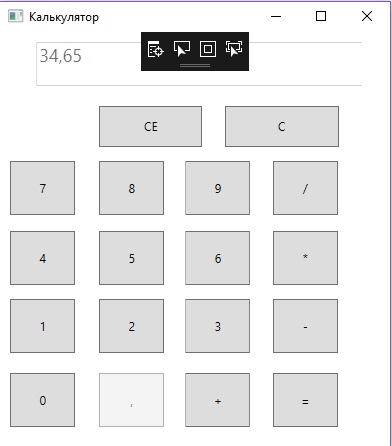
\includegraphics[scale=1.0]{asd}
\caption{Окно программы}
\label{fig:asd}
\end{figure}

\newpage
\textbf{Вывод:} Я научился разрабатывать приложения на WPF;



